% AFOSR Trust and Influence concept white paper; independent of the DTAG manuscript build.
% Source is intentionally self-contained for compilation from DTAG/tex/.
\documentclass[10pt,letterpaper]{article}
\usepackage[T1]{fontenc}
\usepackage{lmodern}
\usepackage{microtype}
\usepackage{geometry}
\geometry{left=0.78in,right=0.78in,top=0.81in,bottom=0.80in}
\usepackage{amsmath,amssymb}
\usepackage{booktabs,tabularx,array}
\usepackage{tikz}
\usetikzlibrary{arrows.meta,positioning,calc,fit}
\usepackage[dvipsnames]{xcolor}
\usepackage{enumitem}
\usepackage{titlesec}
\usepackage{fancyhdr}
\usepackage{hyperref}
\hypersetup{hidelinks,pdftitle={When Questions Change Minds: Trust-Gated Reflexive Dynamics of Influence},pdfauthor={Ishanu Chattopadhyay},pdfsubject={AFOSR Trust and Influence white paper, 2026}}
\definecolor{ink}{HTML}{132A42}
\definecolor{steel}{HTML}{32688A}
\definecolor{teal}{HTML}{087B77}
\definecolor{light}{HTML}{EAF2F3}
\definecolor{graytext}{HTML}{596C78}
\definecolor{pale}{HTML}{F4F7F9}
\newcommand{\kv}[1]{\textbf{\color{ink}#1}}
\newcommand{\order}{\mathrm{order}}
\setlength{\parindent}{0pt}
\setlength{\parskip}{4.7pt}
\setlength{\emergencystretch}{2em}
\titlespacing*{\section}{0pt}{10pt}{3.5pt}
\titleformat{\section}{\sffamily\bfseries\fontsize{11.5}{13}\selectfont\color{ink}}{}{0pt}{}
\titlespacing*{\subsection}{0pt}{7pt}{2pt}
\titleformat{\subsection}{\sffamily\bfseries\fontsize{10.2}{12}\selectfont\color{steel}}{}{0pt}{}
\setlist[itemize]{leftmargin=16pt,topsep=2pt,itemsep=2pt,parsep=0pt}
\pagestyle{fancy}
\fancyhf{}
\fancyhead[L]{\sffamily\fontsize{8}{10}\selectfont\color{steel} AFOSR \textbullet\ TRUST AND INFLUENCE}
\fancyhead[R]{\sffamily\fontsize{8}{10}\selectfont\color{graytext} Research concept \textbullet\ October 2026}
\fancyfoot[L]{\sffamily\fontsize{8}{10}\selectfont\color{graytext} Chattopadhyay \textbar\ University of Kentucky}
\fancyfoot[R]{\sffamily\fontsize{8}{10}\selectfont\color{graytext} \thepage}
\renewcommand{\headrulewidth}{0.45pt}
\renewcommand{\footrulewidth}{0pt}
\begin{document}
\vspace*{-9pt}
{\sffamily\color{teal}\bfseries\fontsize{9.5}{12}\selectfont BASIC RESEARCH WHITE PAPER \hfill FOR PROGRAM DISCUSSION}
\vspace{3pt}

{\sffamily\color{ink}\bfseries\fontsize{20}{22}\selectfont When Questions Change Minds}

{\sffamily\color{steel}\fontsize{13}{16}\selectfont Trust-gated reflexive dynamics in high-dimensional belief systems}
\vspace{3pt}

{\color{graytext}\fontsize{9}{11}\selectfont \textbf{Proposed program:} AFOSR Trust and Influence \quad \textbf{Program officer:} Dr. Laura Steckman\\
\textbf{Principal investigator:} Ishanu Chattopadhyay, University of Kentucky \quad \textbf{Duration:} 36 months}
\vspace{5pt}
\hrule height .7pt
\vspace{5pt}

\section*{The scientific question}
\textbf{When does questioning or trusted information simply reveal a person's existing beliefs, and when does the interaction change the belief system itself?} The distinction remains unresolved because querying a respondent simultaneously supplies a measurement and a cognitive event. A response can reveal a latent disposition, activate a consideration, expose dissonance, or reorganize expectations about other issues. Trust in an information source---human, algorithmic, or institutional---may gate which of these mechanisms operates and whether the response persists.

We propose a \emph{predictive, experimentally falsifiable theory} of such reflexive influence. The project will separate passive statistical updating (learning more about a fixed person) from genuine response or belief-state change, and determine whether trust and prior belief structure predict \emph{resonance, resistance, and recovery}. The ambition is a fundamental science of influence and resilience, not an individualized persuasion system.

\section*{Why AFOSR Trust and Influence}
The AFOSR portfolio prioritizes social/cognitive mechanisms of influence, resonance and dissonance, trust between humans and intelligent agents, and second- or higher-order consequences in heterogeneous information environments [1]. Our hypothesis connects these themes: \emph{source trust changes the response to a local informational perturbation; interdependent beliefs determine where its effects propagate, persist, or dissipate}. Survey-based digital twins supply a measurable baseline against which human influence can be identified rather than presumed. The emphasis is on defensible inference, susceptibility versus resilience, and evaluation of human--AI communication in distributed information settings.

\section*{Technical foundation and preliminary evidence}
In related DARPA MAGICS research, Large Science Models (LSMs) have been used to learn conditional dependencies among high-dimensional survey responses. With 80\% of a defined response set masked, held-out reconstruction reduced mean LSM-distance distortion by approximately \textbf{54.9\% in GSS} and \textbf{60.9\% in Eurobarometer}; over 90\% and 99\% of tested respondents improved, respectively [2]. These are \emph{reconstruction metrics}, not evidence of persuasion.

Our Digital Twin Anchored Generation (DTAG) framework subsequently coupled native LSM conditional response sampling to sequential question selection and an explicit pole-relative ideology geometry [3]. In completed GSS 2024 simulations, six fixed synthetic personas yielded \textbf{960 adaptive ten-question trajectories} and \textbf{2,880 fixed-question-set order replays}. Reordering the same ten items reversed the \emph{direction of simulated ideological displacement} in 131/720 comparisons for right-derived sets and 21/720 for left-derived sets, versus 0/720 for neutral-derived sets. These paired comparisons share baseline realizations and are not independent; a reversal under matched stochastic draws \emph{does not establish different final-state probability laws or changed human beliefs}. Their value is to expose testable model-level order sensitivity and motivate the prospective experiments below.

\vspace{3pt}
\noindent\colorbox{light}{\parbox{\dimexpr\linewidth-2\fboxsep\relax}{\vspace{3pt}\small\color{ink}\textbf{Central hypothesis.} Influence is a state- and trust-dependent perturbation of an interdependent belief system. Conditional geometry forecasts which \emph{unasked} beliefs may respond; randomized human measurements determine which changes reflect construction rather than observation, and whether those changes propagate or recover.\vspace{3pt}}}

\newpage
\section*{Research aims and falsifiable predictions}
\subsection*{Aim 1 \;|\; Distinguish observation from intervention}
Construct an explicit \emph{static refinement null}: a person's unobserved beliefs are fixed and asking additional questions only conditions predictions. Compare it prospectively with an order-sensitive alternative. Consenting participants will be randomized to $A\!\to\!B$, $B\!\to\!A$, $A$-only, $B$-only, and time-matched neutral/no-target controls. Measure outcomes $Y$ in a distinct, previously unasked domain, with a later repeat assessment. The prespecified experimental estimand is
\vspace{-4pt}
\begin{equation}
\tau_{\order}(Y)=\mathbb E\big[Y\mid\operatorname{do}(A\!\to\!B)\big]-
                   \mathbb E\big[Y\mid\operatorname{do}(B\!\to\!A)\big].
\end{equation}
\vspace{-3pt}
\textbf{Falsification:} No order-specific change in held-out outcomes beyond measurement noise or controls, and no prospective predictive gain over conventional psychometric/static models, would reject the proposed dynamic advantage for these question sets.

\subsection*{Aim 2 \;|\; Test trust-gated resonance and resistance}
Introduce balanced, nondeceptive informational material with experimentally varied \emph{verified} human, institutional, or AI provenance; separately measure source trust, perceived credibility, confidence, and nonpolitical behavioral reliance. Where feasible, compare independent text and audio presentations to test whether information-vector changes alter the same response mechanism. Estimate interactions among source trust, baseline opinion geometry, and information--belief congruence. Quantify resonance as a prespecified change in \emph{held-out} beliefs and trust-related behavior, not merely agreement with the presented message. \textbf{Falsification:} If baseline dependency geometry and source trust do not predict out-of-sample heterogeneous response beyond conventional covariates, the hypothesized trust-gated mechanism is unsupported.

\subsection*{Aim 3 \;|\; Measure propagation, resilience, and recovery}
Track direct, adjacent, and deliberately distant \emph{unasked} belief domains; include independent negative controls and remeasurement after 2--4 weeks. Infer whether local exposure has second-order effects, whether changes spread across semantic domains or information vectors, and whether belief configurations return toward baseline. Learn a dynamic transition operator \emph{only from intervention data}, then test its held-out calibration and generalization against the frozen static LSM null. \textbf{Falsification:} Absence of cross-domain or delayed effects, or failure to replicate across cohorts/topics, favors passive refinement or short-lived contextual response rather than durable influence.

\section*{The identification problem in one picture}
\vspace{1pt}
\begin{center}
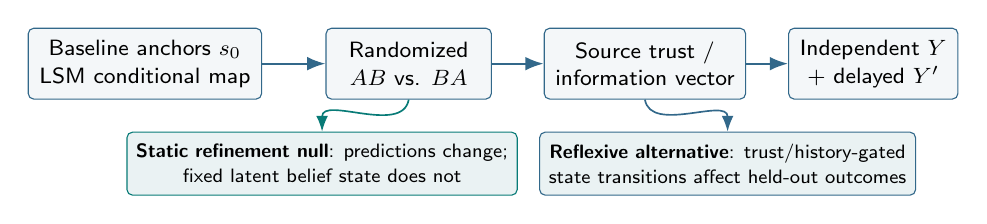
\begin{tikzpicture}[>=Latex,font=\sffamily\fontsize{8}{10}\selectfont,
  box/.style={draw=steel,fill=pale,rounded corners=2pt,align=center,minimum height=9mm,inner sep=4pt},
  arrow/.style={->,thick,draw=steel},
  lab/.style={font=\sffamily\fontsize{7.3}{9}\selectfont,align=center}]
\node[box,minimum width=2.5cm] (base) at (0,0) {Baseline anchors $s_0$\\LSM conditional map};
\node[box,minimum width=2.1cm] (int) at (3.35,0) {Randomized\\$AB$ vs. $BA$};
\node[box,minimum width=2.4cm] (trust) at (6.35,0) {Source trust /\\information vector};
\node[box,minimum width=2.15cm] (out) at (9.25,0) {Independent $Y$\\+ delayed $Y'$};
\draw[arrow] (base)--(int);
\draw[arrow] (int)--(trust);
\draw[arrow] (trust)--(out);
\node[draw=teal,fill=light,rounded corners=2pt,minimum width=4.4cm,minimum height=8mm,lab] (passive) at (2.25,-1.27) {\textbf{Static refinement null}: predictions change;\\fixed latent belief state does not};
\node[draw=steel,fill=light,rounded corners=2pt,minimum width=4.5cm,minimum height=8mm,lab] (dynamic) at (7.4,-1.27) {\textbf{Reflexive alternative}: trust/history-gated\\state transitions affect held-out outcomes};
\draw[->,teal,semithick] (int.south) to[out=-100,in=90] (passive.north);
\draw[->,steel,semithick] (trust.south) to[out=-80,in=90] (dynamic.north);
\end{tikzpicture}
\end{center}
\vspace{-3pt}
\noindent{\footnotesize\color{graytext} \textbf{Figure 1.} The same observed answers can reflect conditioning on an unchanging state or a history-sensitive transition. Random assignment and independently measured, delayed outcomes separate the accounts; DTAG supplies model-derived predictions, not causal labels.}

\newpage
\section*{Measurement, validation, and program of work}
\kv{Pre-registration and identifiability.} Freeze the LSM, conditioning variables, survey-to-model mapping, source-attribution manipulations, experiment arms, held-out outcome domains, and proposed contrasts \emph{before} observing main-study outcomes. Use a participant-disjoint train/validation/test split, blinded comparison against demographic/psychometric and general predictive baselines, and alternate item wording at follow-up to assess measurement invariance. We will compare proper probabilistic scores, confidence intervals of randomized contrasts, calibrated heterogeneity, and multivariate downstream response patterns. An order-induced change in the \emph{sampled DTAG trajectory} alone is not a causal effect.

\kv{Primary human outcomes.} Prespecified composite for independently measured downstream beliefs, source trust and credibility, calibrated confidence, and delayed persistence/recovery. Secondary outcomes include response-time and optional nonpolitical reliance choices. Pilot-derived effect sizes and attrition inform final power; we will report null and negative-control findings. Source trust will be measured rather than inferred from demographic identity. Multiple outcomes and interaction analyses will use prespecified error-rate controls.

\section*{Three-year milestones and decision gates}
\vspace{1pt}
{\fontsize{8.7}{10.8}\selectfont
\renewcommand{\arraystretch}{1.12}
\begin{tabularx}{\linewidth}{@{}p{.70in}X p{2.25in}@{}}
\toprule
\textbf{When} & \textbf{Investigation} & \textbf{Decision gate / product}\\
\midrule
M1--6 & Audit static LSM forecasts, DTAG sensitivity, model provenance; develop preregistered baseline/measurement instruments and ethics submission. & Locked model and data dictionary; ethics-approved pilot protocol before recruitment.\\
M7--12 & Pilot randomized order and trusted-source conditions (planning $N\!\approx\!300$); estimate reliability, attrition, question reactivity and plausible effect sizes. & Power calculation and frozen primary endpoints; go/no-go on confirmatory contrasts.\\
M13--18 & Powered independent-cohort order experiment; assess held-out outcomes and static vs. learned-dynamics forecasts. & Registered randomized-order estimates with CIs; blinded predictive comparison.\\
M19--24 & Trust/provenance and information-vector experiment with 2--4-week follow-up; measure resilience and distant-domain effects. & Tests of resonance, trust moderation, persistence and negative controls.\\
M25--36 & Cross-topic/cohort replication and model comparison; refine or reject transition law according to prospective evidence. & Reproducible protocols, tested theory, publications, deidentified sharable scientific outputs.\\
\bottomrule
\end{tabularx}}

\section*{Novelty, Air Force relevance, and research boundary}
The intellectual contribution is not a new conversational agent but a \emph{quantitative separation between observation and influence}, grounded in high-dimensional conditional statistics and experimentally identified trust/history dependence. The resulting science could improve understanding of human--AI communication, robustness of trust in heterogeneous teams, how ideas reverberate through interdependent beliefs, and why populations or teams resist or recover from informational disruption. The approach does not assume that resonance necessarily implies durable persuasion. Cross-cultural generalization will be evaluated when measurement-compatible cohorts can be recruited; transfer is a hypothesis, not an assertion.

MAGICS supported retrospective modeling and the computational foundation. The proposed AFOSR scope is \emph{new prospective causal human research}, theory validation and generalization, not duplicated support for model construction. Planned term: \textbf{36 months}; preliminary cost range: \textbf{\$200,000--\$250,000 per year}, to be refined with AFOSR guidance and participant-power estimates. Human participation will require institutional review, informed consent, privacy safeguards and nondeceptive materials. No targeting of participants for political susceptibility or operational influence deployment is proposed.

\vspace{3pt}
\noindent\colorbox{light}{\parbox{\dimexpr\linewidth-2\fboxsep\relax}{\small\textbf{Requested program discussion.} We seek Dr. Steckman's feedback on the fit of a hypothesis-driven, three-year Trust and Influence study centered on human experiments, the priority of resonance versus trust-gating, and expectations for a full proposal under the current AFOSR open BAA.}}

\vspace{5pt}
{\footnotesize\color{graytext}\textbf{Selected sources.} [1] AFRL/AFOSR, ``Information and Networks---Trust and Influence,'' program description; AFOSR open BAA FA955026S0001 (2026). [2] Chattopadhyay, DARPA MAGICS Month 4 Technical Report (2026), held-out masked-response reconstruction. [3] DTAG native GSS 2024 computational manuscript and reproducible 10-question persona/order experiments, DTAG repository (2026). [4] Bail et al., ``Exposure to opposing views on social media can increase political polarization,'' \emph{PNAS} 115, 9216--9221 (2018).}

\end{document}